
%\documentclass[notheorems]{beamer}
%\documentclass[handout]{beamer}
%\documentclass[handout,notes=show]{beamer}

%\usepackage[draft]{pdfcomment}

\usetheme{metropolis}

\usepackage{fontspec}
\usefonttheme{professionalfonts} % using non standard fonts for beamer
\setsansfont[
Path           = /Users/alex/Library/Fonts/,
Extension      = .ttf,
Ligatures      = TeX,
UprightFont    = OpenSans-Light,
BoldFont       = OpenSans-Regular,
ItalicFont     = OpenSans-LightItalic,
BoldItalicFont = OpenSans-Italic
]{OpenSans}
\metroset{block=fill}

%\usecolortheme{dolphin}
% No navigation bars 
\beamertemplatenavigationsymbolsempty

\usepackage{amsmath, amssymb, amsfonts, tikz}
\usepackage[utf8]{inputenc}
\usepackage[T1]{fontenc}
\usepackage[english]{babel}
\usepackage{/Users/alex/sage/local/share/texmf/tex/latex/sagetex/sagetex}
\lstdefinestyle{SageInput}{style=DefaultSageInput,numbers=none,basicstyle=\small}
\definecolor{identifiers}{rgb}{0.375,0,0.375}
\definecolor{comments}{rgb}{0.5,0,0}
\definecolor{strings}{rgb}{0,0.5,0}
\definecolor{keywords}{rgb}{0,0,0.5}
\lstdefinestyle{programstyle}{breaklines=true,breakatwhitespace=true,columns=fixed,frame=leftline,framesep=0ex, xleftmargin=0ex,
basicstyle=\tiny\ttfamily,identifierstyle=\color{identifiers},commentstyle=\color{comments},stringstyle=\color{strings},keywordstyle=\color{keywords}}
%% The environments manufactured by the listings package
\lstnewenvironment{programbox}[1][]
  {\lstset{style=programstyle,#1}}
  {}
\lstdefinelanguage{Sage}[]{Python}
{morekeywords={True,False,sage,singular},
sensitive=true}
\definecolor{dblackcolor}{rgb}{0.0,0.0,0.0}
\definecolor{dbluecolor}{rgb}{.01,.02,0.7}
\definecolor{dredcolor}{rgb}{0.8,0,0}
\definecolor{dgraycolor}{rgb}{0.30,0.3,0.30}
\lstset{frame=none,
          showtabs=False,
          showspaces=False,
          showstringspaces=False,
          commentstyle={\ttfamily\color{dredcolor}},
          keywordstyle={\ttfamily\color{dbluecolor}\bfseries},
          stringstyle ={\ttfamily\color{dgraycolor}\bfseries},
          language = Sage,
      basicstyle={\small \ttfamily},
      aboveskip=.3em,
      belowskip=.1em
          }

\usepackage[all]{xy}
\usepackage{wrapfig}
\usepackage{floatrow}
\usepackage{caption}
\usepackage{mathtools}


\graphicspath{{img/}}

\definecolor{Purple}{HTML}{911146}
\definecolor{Orange}{HTML}{CF4A30}
\definecolor{Tan}{RGB}{225,221,191}
\definecolor{Green}{RGB}{76,131,122}
\definecolor{DB}{RGB}{4,37,58}

% Theme colors are derived from these two elements
\setbeamercolor{alerted text}{fg=Green}
\setbeamercolor{frametitle}{bg=Tan,fg=DB}

\metroset{titleformat=smallcaps}


\newtheorem{proposition}[theorem]{Proposition}
\newtheorem{remarks}[theorem]{Remarks}
\newtheorem{remark}[theorem]{Remark}
\newtheorem{conjecture}[theorem]{Conjecture}


\newcommand{\terminology}[1]{\textbf{#1}}

\newcommand{\pdfnote}[1]{\marginnote{\pdfcomment[icon=note]{#1}}}

\newcommand{\NN}{\mathbf{N}}
\newcommand{\ZZ}{\mathbf{Z}}
\newcommand{\QQ}{\mathbf Q}
\newcommand{\CC}{\mathbf C}
\newcommand{\RR}{\mathbf R}
\newcommand{\FF}{\mathbf F}
\newcommand{\dR}{\mathrm{dR}}
\newcommand{\lt}{<}
\newcommand{\gt}{>}
\newcommand{\amp}{&}
\newcommand{\diff}{\mathop{}\!\mathrm{d}}
\newcommand{\ints}{\mathcal{O}}
\newcommand{\ideal}[1]{\mathfrak{#1}}
\usepackage{mathrsfs}\usepackage{cancel}
\newcommand{\Gal}[2]{\operatorname{Gal}(#1/#2)}
\newcommand{\absgal}[1]{\operatorname{Gal}(\overline{#1}/#1)}
\newcommand{\units}{^{\times}}
\DeclareMathOperator{\Spec}{Spec}
\DeclareMathOperator{\Proj}{Proj}

\DeclareMathOperator{\power}{\mathcal{P}}
\DeclareMathOperator{\aff}{\mathbf{A}}
\DeclareMathOperator{\PP}{\mathbf {P}}
\DeclareMathOperator{\norm}{Norm}
\DeclareMathOperator{\trace}{Tr}
\DeclareMathOperator{\Fr}{Fr}
\DeclareMathOperator{\Frob}{Frob}
\DeclareMathOperator{\NS}{NS}
\DeclareMathOperator{\Der}{Der}
\DeclareMathOperator{\Aut}{Aut}
\DeclareMathOperator{\Out}{Out}
\DeclareMathOperator{\Inn}{Inn}
\DeclareMathOperator{\vf}{\mathcal{V}}
\DeclareMathOperator{\krulldim}{krulldim}
\DeclareMathOperator{\trdeg}{trdeg}
\DeclareMathOperator{\Frac}{Frac}
\DeclareMathOperator{\Prob}{Prob}

\newcommand{\sheaf}[1]{\operatorname{\mathcal{#1}}}
\newcommand{\inv}{^{-1}}
\DeclareMathOperator{\Li}{Li}
\DeclareMathOperator{\ord}{ord}
\DeclareMathOperator{\divisor}{div}
\DeclareMathOperator{\Hom}{Hom}
\DeclareMathOperator{\coker}{coker}
\newcommand{\pair}[2]{\left\langle #1, #2 \right\rangle}
\DeclareMathOperator{\characteristic}{char}

\newcommand{\lb}{[}
\newcommand{\rb}{]}

\author{Alex J. Best}
\institute{Boston University}
\date{27/5/2020}
\title{Computations with $p$-adic polylogarithms in Sage}
\subtitle{-- Global Virtual SageDays 109}
\setbeamertemplate{footline}[text line]{\url{https://alexjbest.github.io/talks/sage-computations-polylogs/slides_h.pdf}}

\begin{document}

\begin{frame}
    \titlepage


\end{frame}

%\begin{frame}
%\frametitle{Table of Contents}
%\tableofcontents[currentsection]
%\end{frame}

\begin{frame}{Overview}
    These slides are available online (in handout form) at

    {\url{https://alexjbest.github.io/talks/sage-computations-polylogs/slides_h.pdf}}

    \pdfnote{to read along check, link will be at the bottom of all slides, thank the organisers}\pause

    \textbf{Goal:}  Introduce you to ($p$-adic polylogarithms) in Sage and explain some applications of these computations to solving $S$-unit equations.

\end{frame}

\begin{frame}{What are polylogarithms?}
    Polylogarithms are special functions of a complex variable $z$, obtained by iteratively dividing by $z$ and taking antiderivatives, starting with $\Li_0 = \frac{z}{1-z}$:
    \begin{align*}
        \Li_1 (z) \amp= \int_0^z \frac{t}{(1-t)t} \diff t= - \log(1-z)\text,\\
        \Li_2 (z) \amp= \int_0^z \frac{-\log(1-t)}t \diff t \qquad \text{the \emph{dilogarithm},}\\
        \Li_3 (z) \amp= \int_0^z \frac{\Li_2(t)}t \diff t\\
        \amp\ \ \vdots
    \end{align*}
\end{frame}

\begin{frame}[fragile]{What are polylogarithms?}
    Their power series expansions around zero are rather nice:
    \[\Li_{n}(z)=\sum_{k=1}^{\infty} \frac{z^{k}}{k^{n}}=z+\frac{z^{2}}{2^{n}}+\frac{z^{3}}{3^{n}}+\cdots\]
    (for $|z| < 1$) and we can see that
    \[\Li_n(1) = \zeta (n)\]\pause
    indeed Sage knows this symbolically
    \begin{columns}[c]
        \begin{column}{.5\textwidth}
            \begin{sagecommandline}
                sage: polylog(3, 1)
                zeta(3)
                sage: polylog(2, 1)
                1/6*pi^2
            \end{sagecommandline}
        \end{column}
        \vrule{}
        \begin{column}{.6\textwidth}
            \begin{sagecommandline}
                sage: polylog(2, 1/2)
                1/6*pi^2
                sage: polylog(2, 7.0)
                zeta(3)
            \end{sagecommandline}
        \end{column}
    \end{columns}
\end{frame}

\begin{frame}{Properties of polylogarithms}
    These functions satisfy many interesting functional equations:

    \[\Li_{2}(x)+\Li_{2}(1-x)=\Li_2(1)-\log (x) \log (1-x)\]\pause

    Powering:
    \[\Li_{n}(z^{k}) = \frac{\sum_{m=0}^{k-1} \Li_{n}\left(\zeta _k^mz \right)}{k^{n-1}}\] \pause

    Abel (1826):
    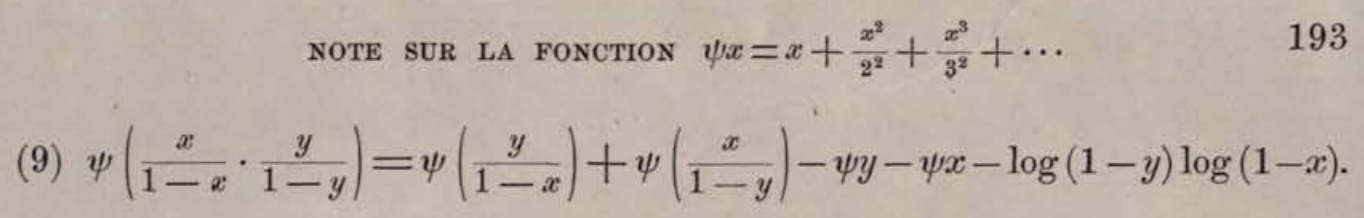
\includegraphics[width=0.9\textwidth]{abel.png}
    \pdfnote{polylogs appear as regulators in K-theory, hyperbolic geometry}
\end{frame}

\begin{frame}{What are the $p$-adics?}
    \pdfnote{In number theory the $p$-adic numbers for primes $p$ play an important role, in}Parallel with the real/complex numbers. They are defined by:

    \begin{enumerate}
        \item Fixing a norm on $\mathbf Q$, defined by \[|x|_p = p^{-\overbrace{\max\{ i \in \ZZ : p^i | x\}}^{=\nu_p(x)}}\]
        \item Completing $\mathbf Q$ with respect to $| \cdot|_p$, to get a complete normed field.
    \end{enumerate} \pause

    Upshot: $p$ is now \emph{small} ($|p|_p = p^{-1}$), so instead of decimal expansions for elements of $\mathbf R$:
    \[\frac13= 3\cdot \frac{1}{10} + 3\cdot \frac{1}{10^2} +  3\cdot \frac{1}{10^3} +  3\cdot \frac{1}{10^4} +  \text{smaller terms}\]
    we have $p$-adic expansions for elements of $\mathbf Q_p$:
    \[\frac13 = 5 + 4 \cdot 7 + 4 \cdot 7^{2} + 4 \cdot 7^{3} + 4 \cdot 7^{4} + \text{smaller terms}\]
\end{frame}

\begin{frame}{$p$-adics in Sage}
    There is now good support for $p$-adics in Sage, thanks to many people, but in particular Xavier Caruso, David Roe and Julian Rüth are regularly working on this (on Zulip).\pause

    Support includes:
    \begin{itemize}
        \item Basic arithmetic
        \item Many different precision tracking modes (absolute / relative, fixed / capped precision)
        \item Hensel lifting (Newton's method)
        \item $\exp$ and $\log$
        \item Frobenius, and Teichm\"uller representatives
        \item Extensions
        \item $\Li_n$?
        \item Much more!
    \end{itemize}
\end{frame}

\begin{frame}{$p$-adic integration}
    To define $\Li_n$, $p$-adically, we must define antiderivatives of $p$-adic functions.

    Easy! Just write out power series locally and take the antiderivative termwise!

    \begin{wrapfigure}{r}{0.30\textwidth}
        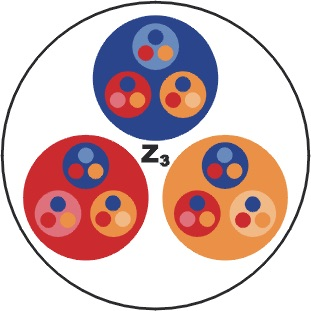
\includegraphics[width=0.9\textwidth]{padic.jpg}
        \caption*{Bad topology!}
    \end{wrapfigure}
    \textbf{Problem:} we can work out local antiderivatives here, and calculate integrals between nearby points, but we can't analytically continue. Distinct disks don't overlap in the $p$-adic topology.
    
    A different constant of integration to be chosen on each $p$-adic disk.
\end{frame}


\begin{frame}{$p$-adic polylogarithms}
    Assume more of the integral, to pin down the function defined: assume Frobenius equivariance:
    \[\int_{x^p}^{y^p} f(t) \diff t= \int_{x}^{y} f(t^p) \diff (t^p) \]\pause
    \emph{For example:} If $f(t) = 1/t$ we can define 
    \[\log (z) \coloneqq \int_1^z\frac{ \diff t}{t}\]
    and find values for $z$ ($p$-adically) near 1 by integrating a power series, \pdfnote{but can't find $\log(-1)$ for instance without Frobenius equivariance}
    \[\log(z^p)= \int_{1}^{z^p} \frac{\diff t}{t} = \int_{1}^{z} \frac{pt^{p-1}\diff t}{t^p} 
    = p\int_{1}^{z} \frac{\diff t}{t} = p\log(z)\]
    so for a $p^k-1$st root of unity $\zeta $ we have\[\log(\zeta ) = \log(\zeta ^{p^k}) = p^k \log(\zeta ) \implies \log(\zeta )= 0\text.\]
\end{frame}

\begin{frame}[fragile]{$p$-adic polylogarithms in Sage}
    Some initial cases (but with restrictions on $p$, $n$, $z$) implemented by Jennifer Balakrishnan (at a Sage days).

    Sage Days 87: $p$-adics in Sage and the LMFDB (2017), I wrote a complete implementation and \href{https://trac.sagemath.org/ticket/20260}{\#20260} was merged.\pause
    \begin{sagecommandline}
        sage: K = Qp(5, prec=7);
    \end{sagecommandline}
    \vspace{-20pt}
    \begin{columns}[c]
        \begin{column}{.55\textwidth}
            \begin{sagecommandline}
                sage: K(1 + 5).polylog(2)
                1
                sage: K(1 + 5^2).polylog(2)
                1
                sage: K(1 + 5^3).polylog(2)
                1
                sage: K(1 + 5^4).polylog(2)
                1
            \end{sagecommandline}
        \end{column}
        \vrule{}
        \begin{column}{.65\textwidth}
            \begin{sagecommandline}
                sage: K(1 + 5^5).polylog(2)
                1
                sage: K(1/2).polylog(2)
                1
                sage: -K(1/2).log()^2/2
                1
                sage: K(7).polylog(3)
                1
            \end{sagecommandline}
        \end{column}
    \end{columns}
    \pdfnote{At the time I had no idea why this was useful!}
\end{frame}

\begin{frame}{How does it work?}
    Besser -- de Jeu: ``$\Li^p $-Service? An Algorithm for Computing $p$-Adic Polylogarithms.'' Math. Comp. 77, no. 262 (2008).

    \begin{itemize}
        \item Near 0: use the power series $\displaystyle\Li_{n}(z)=\sum_{k=1}^{\infty} \frac{z^{k}}{k^{n}}$
        \item Near $\infty $: use the relation
            \[ \Li_{n}(z)+(-1)^{n} \Li_{n}\left(z^{-1}\right)=-\frac{1}{n !} \log ^{n}(z)\]
            to reduce to the first case.\pause
        \item Else: Must be near a $(p^k-1)$st root of unity for some $k$ (except near 1).
            Letting
            \[\Li_{n}^{(p)}(z)=\Li_{n}(z)-\frac{1}{p^{n}} \Li_{n}\left(z^{p}\right)\]
            Reduces to computing $\Li_{m}^{(p)}\left(\zeta^{p^{j}}\right)$ for $m\le n$ and $j<k$.
        \item Near 1: see the paper!
    \end{itemize}

\end{frame}

\begin{frame}{Application: The $S$-unit equation}
    One classic diophantine equation is the $S$-unit equation: for a fixed finite set of primes $S$
    \[u + v = 1,\,u,v\in \QQ^\times\]
    where we ask that the only primes present in the factorization of $u,v$ are those in $S$.

    So
    \[\frac 43 - \frac13 = 1\]
    is a solution of the $\{2,3\}$-unit equation, but not of the $\{2\}$-unit equation or $\{3\}$-unit equation alone.

    The most difficult cases of this equation are when $S$ is large, or over number fields instead.
\end{frame}

\begin{frame}
    In a joint project with Theresa Kumpitsch,  Martin L\"udtke,  Angus McAndrew,  Lie Qian,  Elie Studnia, and Yujie Xu, we have been using $p$-adic polylogarithms (in Sage) to provably determine the full set of solutions to these equations.

    For now only for small $S$, over $\QQ$.\pdfnote{ but we hope to generalize.}
\end{frame}

\begin{frame}{The $S$-unit equation}
    \begin{wrapfigure}{r}{0.4\textwidth}
        \vspace{-25pt}
        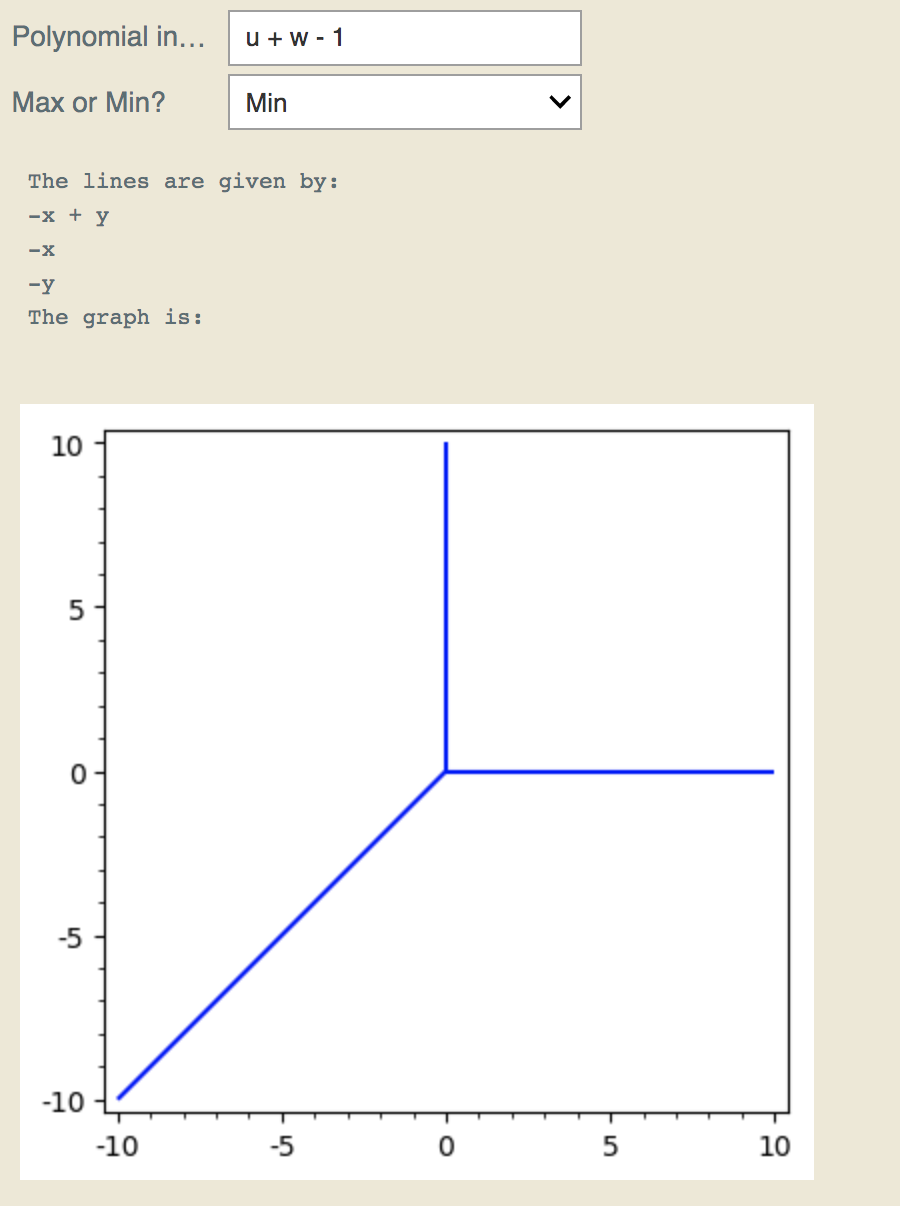
\includegraphics[width=\textwidth]{wang2}
        \caption*{Interact by Wang Weikun}
    \end{wrapfigure}
    Note that for any prime $p$, either $p|u$, $p|v$, or both $p|u\inv$ and $p|v\inv$.

    Plotting $\nu_p(u)$ against $\nu_p(v)$ we get a diagonal Y shape:\pause

    This~is~an~instance~of~a~more general~phenomenon: the valuations lie on the tropical curve associated with the defining equation $u+v=1$.

    \textbf{Note:} If $p \not\in S$ then $u\pmod p$ cannot be any of $0, 1, \infty $.

\end{frame}

\begin{frame}{Applications}
    Minhyong Kim has developed a programme of \emph{non-abelian Chabauty}.

    Extends classical Chabauty's method for finding rational and integral points on curves as zeroes of abelian integrals on the curve.\pause

    One specific consequence of this theory due to Dan-Cohen--Wewers: there exists a commutative diagram for any fixed prime $p$ not in $S$.
    \[\xymatrix{
            \mathbf P^1\smallsetminus\{0,1,\infty\}(\mathbf Z \lb  \frac 1 S \rb )\ar[d]_{(\nu_\ell(z), \nu_\ell(1-z))_{\ell\in S}} \ar[r] & \mathbf P^1\smallsetminus\{0,1,\infty\}(\mathbf Z_p ) \ar[d]^{(\log(z), \log(1-z), -\Li_2(z))} \\
            \aff_{\QQ_p}^{2|S|} \ar@/_/@{->}[r]_{\left(\sum_{\ell \in S} x_\ell \log(\ell),\sum_{\ell \in S} y_\ell \log(\ell), h(\underline x, \underline y)\right)}  & \aff_{\QQ_p}^{3} 
    }\]
\end{frame}

\begin{frame}{Applications}
    In this diagram everything is defined, except $h$, it is a bilinear  form in the $x_\ell$ and $y_\ell$.

    \emph{Strategy:}
    \begin{itemize}
        \item Given enough points in the top $\mathbf P^1\smallsetminus\{0,1,\infty\}(\mathbf Z \lb  \frac 1 S \rb )$, we can find their image in the $\aff^3_{\QQ_p}$ going round the diagram both ways, commutativity then determines $h$.
        \item Given a subvariety $V$ of $\aff^3_{\QQ_p}$ we can find all $S$-units that land in $V$ by pulling back along the right vertical arrow.\pause
        \item Have to solve a polynomial (with $\QQ_p$ coefficients) combinations of $\log(z), \log(1-z),\Li_2(z)$.
        \item To find a useful collection of $V$s covering all possible $S$-units when $|S| =2$ we use the tropical picture, we have 3 components $\{-, |, \diagup\}$ for each prime $\ell \in S$ (Betts--Dogra).
    \end{itemize}
\end{frame}

\begin{frame}[fragile]{Example}
    When $S=\{2,3\}$ we have many solutions
    \[\left\{2, \frac{1}{2}, -1\right\}\cup\left\{ 3,\frac{1}{3},\frac{2}{3}, \frac{3}{2}, -\frac{1}{2}, -2 \right\}\]\[\cup\left\{ 4, \frac{1}{4},  \frac{4}{3},  \frac{3}{4}, -\frac{1}{3},  -3 \right\}\cup\left\{ -\frac{1}{8}, \frac{1}{9}, \frac{9}{8}, \frac{8}{9},9,  -8\right\}\]
    from which we can determine that:
    \[ h =    \tfrac12 \log(2)^2 x_2 y_2 -\Li_2(-2) x_2 y_3 -\Li_2(3)x_3 y_2 + \tfrac12 \log(3)^2 x_3 y_3 \]
\end{frame}

\begin{frame}[fragile]{Example}
    For one choice of $V$ we get that for any $S$-unit $z$ with $2|z$ and $3|(1-z)$ we have
    $\Li_2(-2)\Li_2(z) = \Li_2(3)\Li_2(1-z)$
    which we can solve

    \begin{programbox}[language=Sage]
        sage: allr = allroots(K(1-3).log(p_branch)*K(3).log(p_branch)*Li2z - K(3).polylog(2)*logz*logone_z,p)
        sage: for r in allr:
        ....:    print("root: ",r)
        ....:    print(algdep(r, 2))

        root:  2*5^-1 + 1 + 5^2 + 5^5 + 5^6 + 5^8 + 5^9 + 3*5^11 + 3*5^12 + 4*5^13 + 4*5^14 + 2*5^15 + 4*5^16 + 3*5^17 + 4*5^18 + 2*5^19 + O(5^20)
        11775*x^2 - 119800*x - 28359
        root:  2 + O(5^24)
        x - 2
        root:  2 + 4*5 + 4*5^2 + 4*5^3 + 4*5^4 + 4*5^5 + 4*5^6 + 4*5^7 + 4*5^8 + 4*5^9 + 4*5^10 + 4*5^11 + 4*5^12 + 4*5^13 + 4*5^14 + 4*5^15 + 4*5^16 + 4*5^17 + 4*5^18 + 4*5^19 + 4*5^20 + 4*5^21 + 4*5^22 + 4*5^23 + O(5^24)
        x + 3
        root:  3 + 4*5^23 + O(5^24)
        x - 3
        root:  3 + 5^2 + 2*5^3 + 5^4 + 3*5^5 + 5^6 + 5^7 + 5^9 + 2*5^10 + 3*5^11 + 2*5^12 + 3*5^13 + 3*5^14 + 4*5^15 + 5^16 + 4*5^17 + 3*5^18 + 2*5^22 + 5^23 + O(5^24)
        128901*x^2 - 49672*x - 62943
        root:  4 + 5 + O(5^24)
        x - 9
        root:  4 + 4*5 + 4*5^2 + 4*5^3 + 4*5^4 + 4*5^5 + 4*5^6 + 4*5^7 + 4*5^8 + 4*5^9 + 4*5^10 + 4*5^11 + 4*5^12 + 4*5^13 + 4*5^14 + 4*5^15 + 4*5^16 + 4*5^17 + 4*5^18 + 4*5^19 + 4*5^20 + 4*5^21 + 4*5^22 + 4*5^23 + O(5^24)
        x + 1
    \end{programbox}
\end{frame}
\end{document}
